\section{Zielsetzung}
In diesem Experiment soll eine Dispersionskurve erfasst werden mittels eines Prismas.

\section{Theorie}
Tritt eine Lichtwelle auf eine Grenzschicht, beispielsweise zwischen zwei Medien, dann kommt es zur Wechselwirkung zwischen der Lichtwelle und den
Elektronen und den Ionenrümpfen des Materials. Dabei wird die Lichtgeschwindigkeit der Lichtwelle und dessen Ausbreitungsrichtung verändert. Dieses
Phänomen wird als \textbf{Brechung} bezeichnet. Mit Hilfe des \textbf{Huygensches Prinzip}, welches besagt, dass jeder Punkt einer bestehenden Welle als
Ausgangspunkt einer kugelförmigen Elementarwelle angesehen werden kann und die einhüllende Welle die Wellenfront beschreibt, kann eine Relation
für den \textbf{Brechungsindex} $n$ hergeleitet werden:
\begin{equation*}
  n=\frac{\sin\alpha}{\sin\beta}
\end{equation*}
$\alpha$ und $\beta$ sind in Abbildung \ref{abb:1} dargestellt.
\begin{figure}
  \centering
  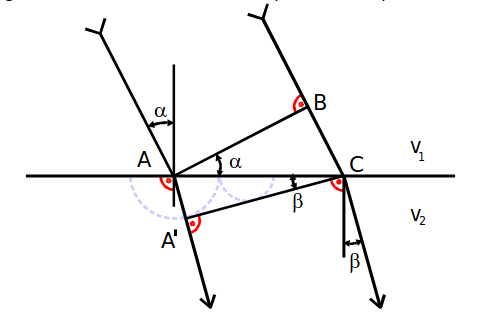
\includegraphics[scale=0.4]{1.png}
  \caption{Darstellung einer gebrochenen Welle an einer Grenzschicht. \cite{Q1}}
  \label{abb:1}
\end{figure}
Der Brechungsindex $n$ beschreibt außerdem die Relation der Lichtgeschwindigkeiten
\begin{equation*}
  n = \frac{v_1}{v_2}
\end{equation*}
dies lässt darauf schließen, dass der Brechungsindex frequenzabhängig sein muss. Die frequenzabhängigkeit des Brechungsindexes wird als \textbf{Dispersion}
bezeichnet. Wenn der Brechungsindex $n$ mit wachsendem $\lambda$ kleiner wird, wird dies als normale Dispersion bezeichnet. Wenn aber der Brechungsindex
bei wachsendem $lambda$ größer wird, wird von einer anormalen Dirpersion gesprochen.

\subsection{Dispersionsgleichung}
Wenn eine Lichtwelle auf eine Grenzschicht trifft, wechselwirkt das elektrische Feld mit den Elektronene und den Ionenrümpfen. Hierbei entstehen mehrere
Kräfte: eine auslenkende, periodische Kraft (durch das elektirsche Feld der eintretenden Welle), eine rücktreibende Kraft (proportional zur Auslenkung), eine
Reinbungskraft (hervorgerufen durch das Medium).
Aus diesen Kräften lässt sich die folgende Differentialgleichung aufstellen:
\begin{equation*}
  \frac{\symup{d^2}\vec{P}_h}{\symup d t^2}+ \frac{f_h}{m_h} \frac{\symup d \vec{P}_h}{\symup d t}+ \frac{a_h}{m_h} \vec{P}_h = \frac{N_q q²_h}{m_h} \vec{E}_0 \symup e^{i \omega t}
\end{equation*}
wobei $\vec{P}_h$ die Polarisation, $m_h$ die Teilchenmasse, $f_h$ die Reibungskonstante, $a_h$ die Federkonstante, $q_h$ die Ladung, $N_h$ die
Ladungsträgerdichte, $E_0$ die Amplitude des elektrischen Feldes der einfallenden Lichtwelle beschreibt und der Index $h$ für das jeweilige Teilchen steht.
Für diese Differentialgleichung ist die Lösung bekannt,
\begin{equation*}
  \vec{P}=\sum\limits_h \frac{1}{\omega_h²-\omega²+i\frac{f_h}{m_h}\omega} \frac{N_q q²_h}{m_h} \vec{E}_0 \symup{e}^{i\omega t} \ \ \ \symup{mit} \ \frac{a_h}{m_h}=\omega².
\end{equation*}
Da die Polarisation in einem Medium der dielektrischen Verschiebung entspricht
\begin{equation*}
  \vec{P} = (\epsilon-1)\epsilon_0 \vec{E}
\end{equation*}
und die Relation $\tilde{n}²=\epsilon$ gilt, kann die Lösung der Differentialgleichung nach dem Brechungindex $n$ umgeformt werden. Außderm muss noch betrachtet
werden, dass $\tilde{n}$ einer komplexen Zahl enspricht, wobei für diesen Versuch nur der Realteil von $\tilde{n}$ von Bedeutung ist. Der Imaginärteil die
Absorptionskonstante beinhaltet. Der reele Anteil $\symup{Re}(\tilde{n})=n$ entspricht dem gesuchten Brechungindex.
Da die Differentialgleichung nur eine Näherung für das Problem beschreibt, müssen zunächst Annahmen für die Gültigkeit dieser gemacht werden. Eine dieser
Annahmen ist, dass die Gleichung nicht in der Nähe der Absortionsfrequenzen durchgeführt wird, also das $\lambda << \lambda_1$ oder $\lambda >> \lambda_1$ gilt,
diese wird in dem Experiment damit erfüllt, dass wir im Bereich des sichtbaren Lichtes liegen und dort keine Absorptionsfreuquenzen des verwendeten Materials liegen.
Mit dieser Bedingung, kann $n²k \approx 0$ angenommen werden. Daraus folgt für den Brechungsindex:
\begin{equation}
  \label{eq:1}
  n²(\lambda)=1+ \frac{N_1 q_1²}{4\pi² c² \epsilon_0 m_1} \frac{\lambda_1²}{{1-\left(\frac{\lambda_1}{\lambda}\right)²}}
\end{equation}
Mittels dieser Formel kann jetzt eine Fallunterscheidung durchgeführt werden:
\begin{itemize}
  \item $\lambda << \lambda_1$: Liegt die Resonanzstelle also über der Messstelle, kann die Gleichung \eqref{eq:1} mittels einer Taylorentwicklung vereinfacht
  werden. Die dabei entstehende Kurve ist in Abbildung \ref{abb:2} b) abgebildet.
  \begin{equation*}
    n²(\lambda) = 1+\frac{N_1 q²_1 \lambda_1²}{4 \pi c² \epsilon_0 m_1} \left(1+\left(\frac{\lambda_1}{\lambda}\right)²+\left(\frac{\lambda_1}{\lambda}\right)⁴+ ...\right)
  \end{equation*}
  mit den Koeffizienten $A_i>0$:
  \begin{equation}
    \label{eq:2}
    n²(\lambda) = A_0 + \frac{A_2}{\lambda²}+\frac{A_4}{\lambda⁴}+...
  \end{equation}
  \item $\lambda >> \lambda_1$: Liegt die Resonanzstelle unter der Messstelle, kann die Gleichung \eqref{eq:1} erneut mittels einer Taylorentwicklung vereinfacht
  werden. Die dabei entstehende Kurve ist in Abbildung \ref{abb:2} a) abgebildet.
  \begin{equation*}
      n²(\lambda) = 1-\frac{N_1 q¹_1}{4 \pi c² \epsilon_0 m_1} \left(\lambda²+\frac{\lambda⁴}{\lambda_1^2}+\frac{\lambda⁶}{\lambda_1^4}+...\right)
  \end{equation*}
  und mit den Koeffizienten $A'_i>0$:
  \begin{equation*}
    n²(\lambda) = 1-A'_2\lambda²-A'_4\lambda⁴-...
  \end{equation*}
\end{itemize}
\FloatBarrier
\begin{figure}
  \centering
  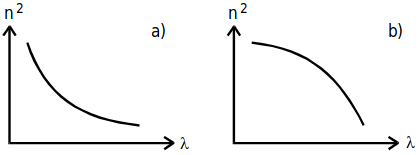
\includegraphics[scale=0.6]{2.png}
  \caption{Dispersionskurven für a) $\lambda >> \lambda_1$ und b) $\lambda << \lambda_1$. \cite{Q1}}
  \label{abb:2}
\end{figure}
\FloatBarrier

\section{Durchführung}
Der Versuch setzt sich aus zwei Teilen zusammen, zunächst wird der Winkel des Prismas gemessen, an dem die Strahlen gebrochen werden. Im zweiten Teil des Versuchs
soll die Dispersionkurve gemessen werden.

\subsection{Aufbau}
Das Kernstück des Versuches ist ein Prismenspektralapparat, dieser ist in Abbildung \ref{abb:3} schematisch dargestellt.
\begin{figure}
  \centering
  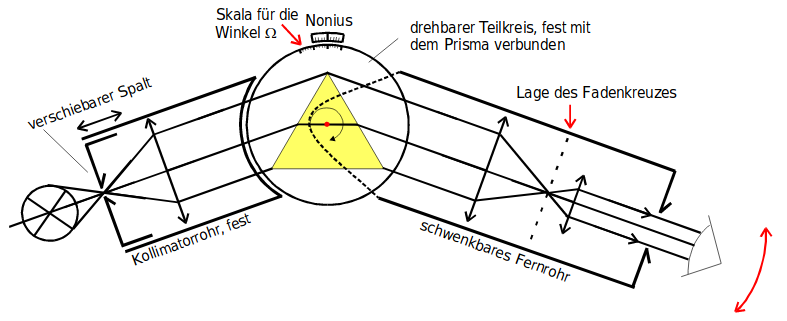
\includegraphics[scale=0.4]{3.png}
  \caption{Schematischer Aufbau eines Prismenspektralapparats. \cite{Q1}}
  \label{abb:3}
\end{figure}
Durch ein Quecksilberlampe wird das zu untersuchende Licht erzeugt. Dieses wird durch eine Blende und ein Kollimatorrohr gebündelt, sodass dieses parallel verläuft.
Daraufhin wird das Licht durch ein bewegliches Prisma geschickt, wobei der Winkel des Prismas an einer Skala abgelesen werden kann. Wurde das Licht durch das Prisma
nun in seine Spektralfarben zerlegt, verläuft es jetzt durch ein schwenkbarer Fernrohr. Hier lassen sich die Spektralfarben mit hilfe eines Fadenkreuzes beobachten.

Im ersten Verscuhteil soll der Winkel des Prismas gemessen werden. Hierzu wird das Prisma auf dem bewegliches Teller so ausgerichtet, dass die zu messende Ecke
in Richtung der Lampe zeigt. Jetzt wird mit hilfe des schwenkbaren Fernrohr die reflektierten weißen Linien gesucht und deren Winkelabstand gemessen. Nun wird das
Prisma auf dem Teller leicht verschoben und erneut gemessen. Diese Messung wird insgesamt 5 mal durchgeführt.

Im zweiten und letzten Versuchsteil soll nun eine Dispersionskurve dargestellt werden. Die schematische Darstellung der Messung ist in Abbilung \ref{abb:4} dargestellt,
der kleinste Winkel des abgebildeten Prismas ist hierbei der Winkel, der zuvor im ersten Versuchteil vermessen wurde. Zunächst wird das Prisma so aufgestellt, dass
die Vermessene Ecke nach rechts zeigt. Jetzt wird so lange an dem Teller und an dem Fernrohr gedreht, bis die weiße Linie deckungsgleich mit der zu vermessenden
Spektrallinie liegt. Der Winkel $\Omega_l$, bei dem dies der Fall ist, wird notiert. Dies wird für alle Spektrallinien durchgeführt. Auf der anderen Seite wird dies
für alle Spektrallinien wiederholt und der Winkel $\Omega_r$ gemessen. Hierbei muss die vermessene Ecke des Prismas nach links außen zeigen. Die Ausrichtung der
Nulllinie spielt keine Rolle, da nur die Winkeldifferenzen von Bedeutung sind.

\begin{figure}
  \centering
  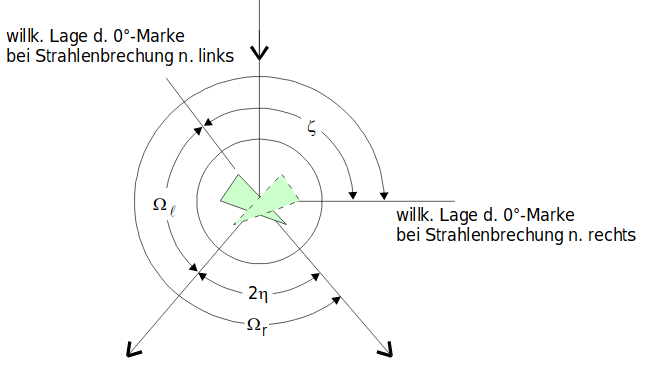
\includegraphics[scale=0.4]{4.png}
  \caption{Schematische Darstellung der zweiten Messung. \cite{Q1}}
  \label{abb:4}
\end{figure}

\section{Auswertung}
\subsection{Bestimmung des brechenden Winkels.}
Im ersten Teil des Versuchs wird der brechende Winkel $\varphi$ bestimmt. Dies geschieht, indem die beiden reflektierten Strahlen
$\varphi_{\symup{l}}$ und $\varphi_{\symup{r}}$ gemessen werden. Die Messergebnisse sind zusammen mit den nach Formel \ref{eq:1} berechneten
Werten für den brechenden Winkel in Tabelle \ref{tab1} zu sehen.
Die Mittelung der sieben Messwerte, sowie der zugehörige Fehler für die Mittelung werden mit Hilfe folgender Formeln berechnet:
\FloatBarrier
\begin{align*}
  \bar{\varphi} &= \frac{1}{n} \sum_{1}^{7}{\varphi_n}  \\
  \upsigma &= \frac{1}{\sqrt{n}} \sqrt{\frac{\sum{(\varphi_n - \bar{\varphi})^2}}{n-1} }
\end{align*}
\FloatBarrier
\begin{table}
\centering
\caption{Messwerte und Ergebnisse zur Ermittlung von $\varphi$}
\label{tab1}
\begin{tabular}{ c c c c }
\toprule
{Messung} & { $\varphi_{symup{l}}$ / $\si{\degree}$ } & { $\varphi_{symup{r}}$ / $\si{\degree}$ } & { $\varphi$ / $\si{\degree}$ } \\
\midrule
 1 & 69,6   &   189,6   &   60,00   \\
 2 & 71,1   &   191,2   &   60,05   \\
 3 & 68,9   &   189,0   &   60,05   \\
 4 & 63,0   &   183,0   &   60,00   \\
 5 & 63,5   &   183,6   &   60,05   \\
 6 & 61,0   &   180,9   &   60,05   \\
 7 & 62,6   &   182,6   &   60,00   \\
\bottomrule
\end{tabular}
\end{table}
Für $\bar{varphi}$ ergibt sich ein Wert von $\SI{60,03(1)}{\degree}$.
\subsection{Bestimmung des Brechungswinkels und der Brechungsindizes n}
\noindent Im darauffolgenden Teil des Versuchs wird der Winkel $\eta$, sowie die Brechungsindizes für die verschiedenen Wellenlängen berechnet.
Die hierfür benötigten Werte sind in Tabelle \ref{tab2} zu sehen.
\begin{table}
\centering
\caption{Messwerte zur Bestimmung von $\eta$ und n}
\label{tab2}
\begin{tabular}{ c c c c c }
\toprule
{Wellenlänge} & {$\Omega_{l}$ / $\si{\degree}$ } & { $\Omega_{r}$ / $\si{\degree}$ } & { $\eta$ } & { n }\\
\midrule
 643,84     &     192,0     &     70,0      &      58,0     &     1.71383 \pm 0.00017     \\
 576,96     &     191,7     &     70,5      &      58,8     &     1.72097 \pm 0.00017     \\
 546,07     &     191,3     &     70,7      &      59,4     &     1.72627 \pm 0.00017     \\
 508,58     &     190,9     &     71,2      &      60,3     &     1.73414 \pm 0.00017     \\
 479,99     &     190,5     &     71,7      &      61,2     &     1.74189 \pm 0.00017     \\
 467,81     &     190,3     &     71,8      &      61,5     &     1.74446 \pm 0.00017     \\
 435,83     &     189,8     &     72,4      &      62,6     &     1.75375 \pm 0.00017     \\
\bottomrule
\end{tabular}
\end{table}
Die Brechungsindizes n werden mit Hilfe folgender Formel berechnet:
\begin{align*}
  \symup{n} = \frac{\symup{sin}(\frac{\upeta + \varphi}{2})}{\symup{sin}(\frac{\varphi}{2})}
\end{align*}
Der zugehörige Fehler berechnet sich mit
\begin{align*}
  \Delta \symup{n} = \bigg\vert\bigg(\frac{0,5 \symup{cos}(\frac{n+\varphi}{2})}{\symup{sin}(\frac{\varphi}{2})} - \frac{0,5 \symup{cos}(\frac{\varphi}{2})\symup{sin}(\frac{n+\varphi}{2})}{\symup{sin^2}(\frac{\varphi}{2})}\bigg)\Delta \varphi\bigg\vert  .
\end{align*}
\FloatBarrier
\subsection{Ermittlung der Dispersionsgleichung}
\noindent Im folgenden wird untersucht, welche Theoriekurve zur Ermittlung der Dispersionsgleichung genauer den genommenen Messwerten entspricht.
In Abbildung \ref{abb1} sind die quadrierten Brechungsindizes $\symup{n}^2$ gegen ihre Wellenlängen aufgetragen. In derselben Abbildung sind
die beiden Theoriekurven zu sehen. Es deutet sich an, dass Theoriekurve 1 die Messwerte genauer trifft als Theoriekurve 2.
Die mit Hilfe der Theoriekurven ermittelten ersten beiden Koeffizienten für die Dispersionsgleichungen 1) und 2) sind in Tabelle \ref{tab3}
zu sehen.
\FloatBarrier
\begin{table}
\centering
\caption{Koeffizienten der Dispersionsgleichung.}
\label{tab:disp}
\begin{tabular}{ c | c c }
\toprule
{Dispersionskurve} & & {Steigung} \\
\midrule
  1 & $\symup{A_0}$   & $\num{2,812(5)}$      \\
      & $\symup{A_2}$ & $\num{5,05(13)E4}$    \\
  2 & $\symup{A_0'}$  & $\num{3,165(14)}$     \\
      &$\symup{A_2'}$ & $\num{5,8(5)E-7}$     \\
\bottomrule
\end{tabular}
\end{table}
\FloatBarrier
Mit Hilfe der ermittelten Koeffizienten lassen sich nun die Abweichungsquadrate berechnen:
\begin{align*}
  \symup{s}_{\symup{n}}^2 &= \frac{1}{5} \sum\limits_{i=1}^{7} \left( \symup{n}^2( \lambda_{\symup{i}} ) - \symup{A_0} - \frac{\symup{A_{2}}}{\lambda_{\symup{i}}^2} \right)^2  \\
  \symup{s}_{\symup{n'}}^2 &= \frac{1}{5} \sum\limits_{i=1}^{7} \left( \symup{n'}^2( \lambda_{\symup{i}} ) - \symup{A_0'} + \symup{A_{2}'} \lambda^2 \right)^2
\end{align*}
Es wird der Gleichung die Gültigkeit zugesprochen, die ein kleineres ${\symup{s}}^2$ besitzt.
Die Abweichung für $\symup{s}_\symup{n}$ beträgt $\SI{6,2(25)E-6}{}$, wohingegen die Abweichung für $\symup{s}_{\symup{n'}} \SI{190(70)E-6}{}$ beträgt.
Dies lässt darauf schließen, dass die Theoriekurve 1 den Messwerten exakter entspricht.
Somit ergibt sich für den Brechungsindex des verwendeten Glasprismas in Abhängigkeit von der Wellenlänge folgende Gleichung:
\begin{align*}
  \symup{n}(\lambda) = \sqrt{ \symup{A_0} + \frac{\symup{A_2}}{\lambda ^2} }
\end{align*}
\FloatBarrier
\begin{figure}
  \centering
  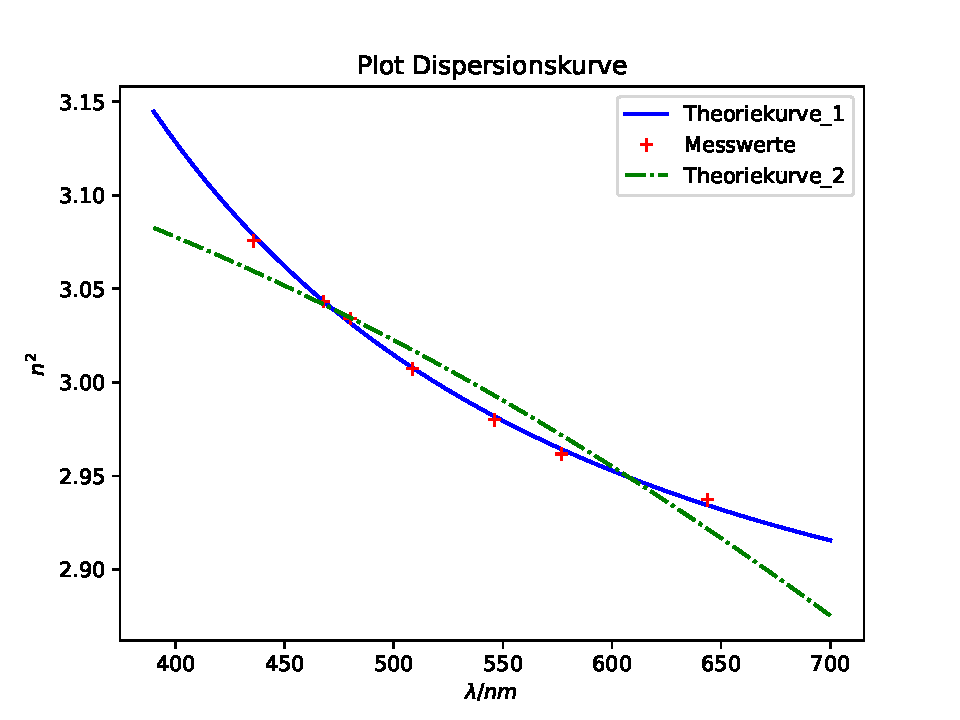
\includegraphics[scale=0.5]{dispersion.pdf}
  \caption{Vergleich der Theoriekurven mit den Messergebnissen.}
  \label{abb1}
\end{figure}
\subsection{Berechnung der Abbe'schen Zahl}
Mit Hilfe dieser Gleichung lässt sich die Abbesche Zahl einfach über folgende Formel berechnen:
\begin{align*}
  \nu = \frac{\symup{n}_\symup{D} - 1}{\symup{n}_\symup{F} - \symup{n}_\symup{C}}
\end{align*}
\FloatBarrier
Hierbei sind die Wellenlängen für die Frauenhoferschen Linien wie folgt angegeben:
\begin{align*}
  \lambda_\symup{D} &= \SI{589}{\nano \metre} \\
  \lambda_\symup{F} &= \SI{486}{\nano \metre} \\
  \lambda_\symup{C} &= \SI{656}{\nano \metre}
\end{align*}
Folglich ergibt sich eine Abbe'sche Zahl von $\SI{25,8(6)}{}$. Der Fehler für die Abbe'sche Zahl entsteht dadurch, dass in der Berechnung der
Brechungsindizes fehlerbehaftete Größen vorkommen, weshalb diese ebenfalls wieder fehlerbehaftet sind. Die Fehler für die Brechungsindizes werden
mittels Gauß'scher Fehlerfortpflanzung berechnet. Folglich ergeben sich folgende Werte für die Brechungsindizes:
\begin{align*}
  \symup{n}_\symup{D} &= \SI{1,7198(18)}{\nano \metre} \\
  \symup{n}_\symup{F} &= \SI{1,7395(21)}{\nano \metre} \\
  \symup{n}_\symup{C} &= \SI{1,7115(17)}{\nano \metre}
\end{align*}

\subsection{Auflösevermögen}
Das Auflösevermögen beschreibt den minimalen Wellenlängenunterschied $\Delta \lambda$, der zwischen zwei Spektrallinien liegen darf, damit sie
vom Gerät gerade noch getrennt werden können.
Es ist definiert als:
\FloatBarrier
\begin{align*}
  \symup{A} := \frac{\lambda}{\Delta{\lambda}}
\end{align*}
Woraus dann die Formel zur Berechnung des Auflösevermögens folgt:
\FloatBarrier
\begin{align*}
  \symup{A} &= \symup{b} \frac{\symup{dn}}{\symup{d}\lambda} \\
            &= -\symup{b} \frac{\symup{A_2}}{\sqrt{\symup{A_0} + \frac{\symup{A_2}}{\lambda^2}}\lambda^3}
\end{align*}
Da auch hier wieder fehlerbehaftete Größen zur Berechnung verwendet werden, muss die Gauß'sche Fehlerfortpflanzung beachtet werden und es wird
der Fehler von A mittels folgender Formel berechnet:
\begin{align*}
  \Delta{A}= \sqrt{\left[\left(-\frac{\symup{bA_2}}{\lambda^3}\cdot0,5\left(\symup{A_0}+ \frac{\symup{A_2}}{\lambda^2}\right)^{-\frac{3}{2}}\right)\Delta{A_0}\right]^2+\left[\frac{\symup{b}}{\lambda^3}\left(\symup{A_0}+\frac{\symup{A_2}}{\lambda^2}\right)^{-\frac{1}{2}}\cdot\left(\frac{-\symup{A_2}}{2\lambda^2}\left(\symup{A_0}+\frac{\symup{A_2}}{\lambda^2}\right)^{-1}+1\right)\right]^2}
\end{align*}

\noindent Für die drei zuvor verwendeten Frauenhofer'schen Linien ergeben sich, die in Tabelle \ref{tab3} zu sehenden Ergebnisse für das
Auflösungsvermögen.
\FloatBarrier
\begin{table}
\centering
\caption{Auflösevermögen für die Fraunhoferschen Linien.}
\label{tab3}
\begin{tabular}{ c c c }
\toprule
{ Fraunhofersche Linie } & { $\lambda$ / $ \si{\nano \metre} $ } & { Auflösevermögen } \\
\midrule
 $\lambda_{\symup{C}}$ & 656 & $\SI{3140(80)}{} $     \\
 $\lambda_{\symup{D}}$ & 589 & $\SI{4310(110)}{}$     \\
 $\lambda_{\symup{F}}$ & 486 & $\SI{7590(190)}{}$     \\
 \bottomrule
\end{tabular}
\end{table}
\FloatBarrier
\subsection{Bestimmung der nächstgelegenen Absorptionsstelle}
Um die nächstgelegene Absorptionsstelle zu ermitteln, wird ein Koeffizientenvergleich der beiden Gleichungen \ref{eq:1} und \ref{eq2} durchgeführt:
\begin{align*}
  \lambda_1 = \sqrt{\frac{\symup{A_2}}{\symup{A_0} -1}}.
\end{align*}
Der zugehörige fehler berechnet sich mittels folgender Formel:
\begin{align*}
  \Delta{\lambda} = \sqrt{\left(\frac{1}{2}\left(\frac{\symup{A_2}}{\symup{A_0}-1}\right)^{-\frac{1}{2}}\frac{1}{\symup{A_0}-1}\Delta{\symup{A_2}}\right)^2 + \left(\frac{1}{2}\left(\frac{\symup{A_2}}{\symup{A_0}-1}\right)^{-\frac{1}{2}}\frac{{-\symup{A_2}}}{(\symup{A_0}-1)^2}\Delta{A_0}\right)^2}.
\end{align*}
Somit ergibt sich für die nächstgelegene Absorptionsstelle eine Wellenlänge von $\SI{166,9(22)}{\nano \metre}$.
Diese Wellenlänge liegt im stark ultravioletten Bereich \cite{Q2}.
\section{Diskussion}
Die Bestimmung des brechenden Winkels $\varphi$ = $\SI{60,03(1)}{\degree}$ weist eine sehr geringe Abweichung von $\SI{0,05}{\percent}$ auf,
was im Rahmen der Messungenauigkeit liegt.
Bei der Ermittlung des Winkels $\upeta$ konnten leicht Fehler geschehen. So war es recht schwer zu erkennen, wann die reflektierte Linie über
den zu vergleichenden Spektrallinien lag, weil sich diese durch das Vertsellen des Goniometers leicht verschieben ließen.
Das Verhalten der normalen Dispersion ist jedoch deutlich zu erkennen. Bei abnehmenden Wellenlängen steigen die Brechungsindizes an.
Der Brechungsindex n des Materials SF14 beträgt $1,756$ bei einer Wellenlänge von $\SI{632,8}{\nano \metre}$ \cite{Q3}.
Der berechnete Wert beträgt $1,714$, was einer prozentualen Abweichung von $\SI{2,40}{\percent}$ entspricht. Dies spricht dafür, dass keine
systematischen Fehler bei der Durchführung gemacht wurden. Der Literaturwert für die Abbe'sche Zahl beträgt $26,50$, von dem der experimentell
ermittelte Wert von $25,8$ um $\SI{2,64}{\percent}$ abweicht.
Es ist davon auszugehen, dass die berechnete Dispersionskurve, als auch die ermittelten Paramter der Realität sehr nahe kommen.
